%  Copyright 2020-2024 Robert Bosch GmbH
%
%  Licensed under the Apache License, Version 2.0 (the "License");
%  you may not use this file except in compliance with the License.
%  You may obtain a copy of the License at
%
%      http://www.apache.org/licenses/LICENSE-2.0
%
%  Unless required by applicable law or agreed to in writing, software
%  distributed under the License is distributed on an "AS IS" BASIS,
%  WITHOUT WARRANTIES OR CONDITIONS OF ANY KIND, either express or implied.
%  See the License for the specific language governing permissions and
%  limitations under the License.

\chapter{Logging}

\section{Background}

The \rfwcore\ provides several log levels (also known as trace levels) to give users the possibility to control the amount of output in log files.
The build in keyword \rcode{log} writes content to the log files. The optional parameter \rcode{level} of this keyword defines under which conditions
(under which log level) the \rcode{log} keyword shall write the log message.

With command line parameter \rlog{--loglevel} a user defines this condition. If the log level of an executed \rcode{log} keyword matches to the
log level defined for test execution, the log message is logged, otherwise not.

Available log levels in \rfwcore\ are: \rcode{ERROR}, \rcode{WARN}, \rcode{INFO}, \rcode{DEBUG} and \rcode{TRACE}.
The default log level in \rfwcore\ is \rcode{INFO}. This level becomes active, if nothing else is specified by a user.

The log level \rcode{INFO} is also used by the \rfwcore\ itself, e.g. for the logging of informations about executed keywords.
The impact is that every log file contains both the users output and the \rfwcore\ output.
For larger tests this might cause unfavorable large log files.

Therefore the \rfw\ provides an additional log level \rcode{USER}. Tests that are executed under this log level, do not contain
the \rfwcore\ \rcode{INFO} messages any more (but for sure still contain errors and warnings).

\textbf{Example code:}

\begin{robotcode}
log    my log message    USER
\end{robotcode}

\textbf{Example execution:}

\begin{robotlog}
python -m robot --loglevel USER -b logfile.log ./testfile.robot
\end{robotlog}

\section{Summary}

In opposite to the \rfwcore\ (core), the \rfw\ provides the following log levels to control the amount of logged content:

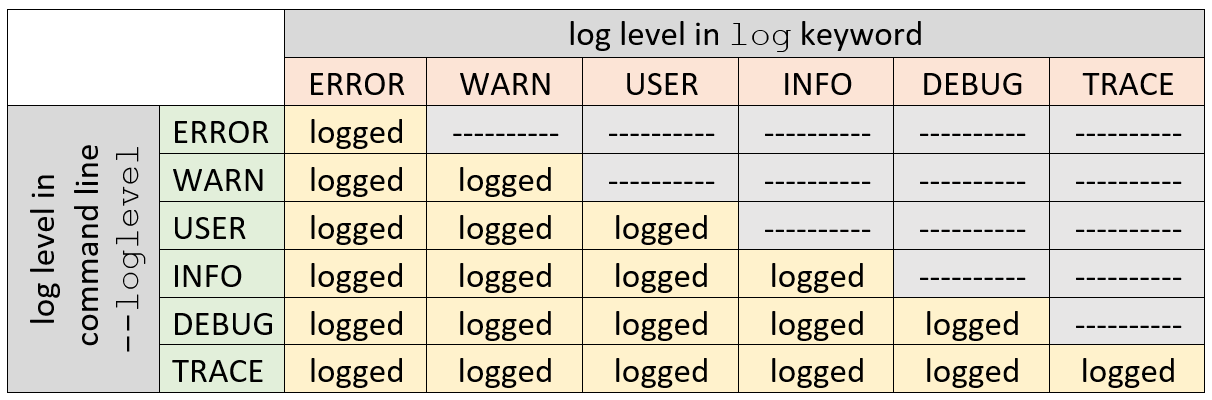
\includegraphics[scale=0.7]{./include/graphics/logging/LogLevelTable}

The log level \rcode{USER} has been added to give users the possibility to log own content without all \rcode{INFO} messages logged by the \rfwcore\ (core).

